%%%%%%%%%%%%%%%%%%%%%%%%%%%%%%%%%%%%%%%%%%%%%%%%%%%
%
%  New template code for TAMU Theses and Dissertations starting Fall 2016.
%
%
%  Original Author: Sean Zachary Roberson
%  This version adapted for URS by Parasol lab.
%  Adapted from version 3.16.10, which was last updated on 9/29/2016.
%  URS adaptation last updated 1/9/2017.
%
%%%%%%%%%%%%%%%%%%%%%%%%%%%%%%%%%%%%%%%%%%%%%%%%%%%
%%%%%%%%%%%%%%%%%%%%%%%%%%%%%%%%%%%%%%%%%%%%%%%%%%%%%%%%%%%%%%%%%%%%%%%
%%%                           ALGORITHM
%%%%%%%%%%%%%%%%%%%%%%%%%%%%%%%%%%%%%%%%%%%%%%%%%%%%%%%%%%%%%%%%%%%%%%

\chapter{THE ALGORITHM}


\section{Introduction}

The core portion of the platform that will allow reordering of aspects of the textbook can simply summed up as \textit{The Algorithm}. This underlying algorithm is independent of technology stack or implementation. It is simply a high level description and analysis of the proposed solution to the given problem.

With simply an understanding of the algorithm, the implementation should follow in a natural and simple manner.

\section{Motivation for the Algorithm}

The algorithm has other items to consider outside simply just solving the given issue. As with most algorithms, there is a thought and focus on completing the desired task in an efficient and optimal manner. This means that if the algorithm is able to provide feedback but if it is done in an clunky manner, the algorithm is still considered a failure and not useful.

In addition to efficiency, correctness is another major point of focus. In this context, correctness relates to properly conveying the thoughts and concerns of the original author to the professor or institution trying to modify the ordering of a textbook. As a result of a particular action or modification by the consumer, there should never arise a situation where a suggestion or warning provided by the algorithm conflicts with the thoughts or viewpoints of the original author of the textbook. These messages provided by the algorithm should be simply an extension of the original if not exactly the same as if the author was at the computer sitting with the user of the platform.

Correctness also relates to truly reordering the textbook as desired and specified by the one who modified the order of the textbook. After a change by the consumer, they should be able to clearly understand what type of change they are proposing, how this affects the textbook as a whole, how nearby sections or chapters may be affected and finally after committing these changes, the actual textbook should properly reflect these changes as desired by the consumer. 

\section{The Design}

\subsection{Structure}

The design first has to answer the question of what. What information is necessary  to properly accomplish the given task. There are N items that are being considered. At the root of everything, there is a topic. This is the core dependency upon which all other dependencies are built upon or contrived from. All the following data types all directly or indirectly are tied to a particular topic or group of topics. A unit is very generic and could be broken up into three different types. A unit is either a chapter, section or page. For the purpose of dependency mapping, there has not been a use case that distinctly separates one of these from another for the purpose of dependency mapping so therefore they have been simply grouped together into type unit. The final data type is exercise. An exercise is different than a unit because of how it is presented and how the underlying content is used. A unit is simply a presentation of content and/or topics to the reader. An exercise is formal way of testing the consumers knowledge and practice their skills. Another special consideration of exercises is their dynamic and flexible nature. Unit structure is what the consumer will likely spend a majority of time reordering and tweaking. Once the unit structure is in place, the exercises should automatically populate and relate to the correct units given the new unit dependency mapping.

The next topic of focus is how to properly structure the necessary information to complete the given task. Since this is in fact a hierarchical dependency mapping problem at its core, a directed acyclic graph (DAG) is the format was chosen to map and store the dependencies. The reason being because a given topic can have one of two true relations and one metarelation with any another topic. This given topic may depend on another topic because material must first be introduced in the latter topic in order to properly deliver the content in the former topic. This is an example of a child relationship. The reverse relation is also a relationship. This reverse relationship is an example of a parent relationship \ref{fig:parent_child}.

\begin{figure}[ht]
    \centering
    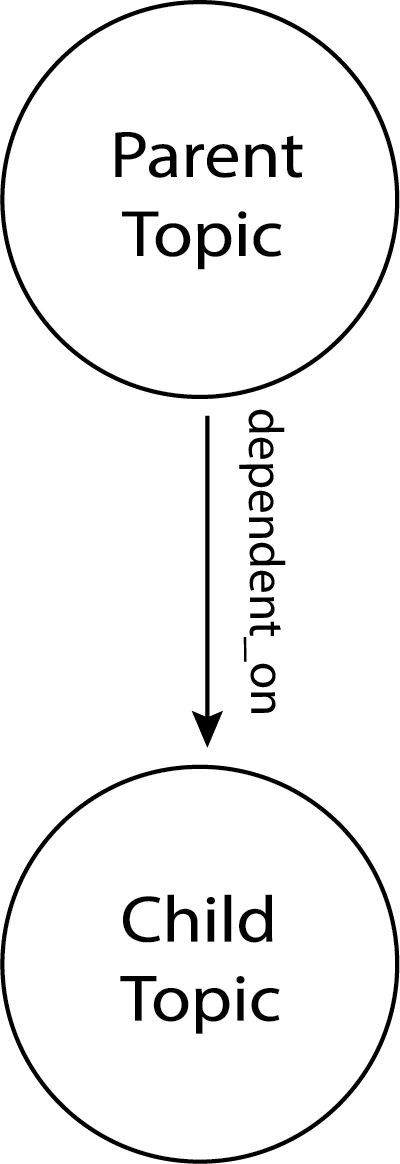
\includegraphics[scale=0.75]{parent_child.png}
    \caption[parent child topic.]{Parent child topics.}

    \label{fig:parent_child}
\end{figure}

Finally, the metarelation is the situation where two topics are located on similar levels of the hierarchy in the dependency mapping and do not have a parent or child relationship with one another. These topics are independent of one another, meaning that the order of these two topics in no way affect one another \ref{fig:unrelated_topics}.

\pagebreak
\begin{figure}[ht]
    \centering
    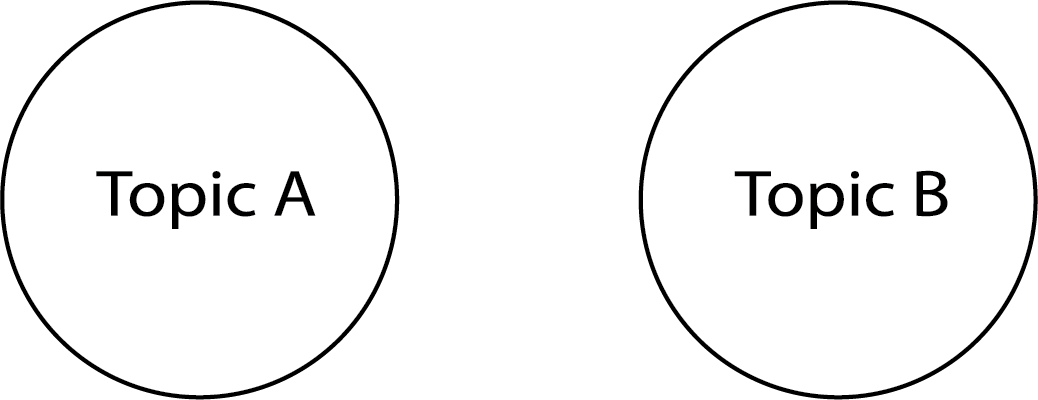
\includegraphics[scale=0.75]{unrelated_topics.png}
    \caption[Unrelated topics.]{Unrelated topics. Can have any number of parents and children but do not relate to one another.}
        
    \label{fig:unrelated_topics}
\end{figure}

The previous dependency mapping completely describes the requirements for mapping topics but units and exercises require more mapping. Units have two relationships to map too. Like topics, units have a dependency mapping between the same types as themselves. Units are also tied to topics because units are the form in which topics are introduced in the textbook. A particular unit can introduce one more topics. For the purpose of relating these two, an unique id is assigned to each topic. For a given chapter then depends on $N$ topics, a list of unique ids of each of the $N$ topics are stored on the chapter node \ref{fig:units}.

\begin{figure}[ht]
    \centering
    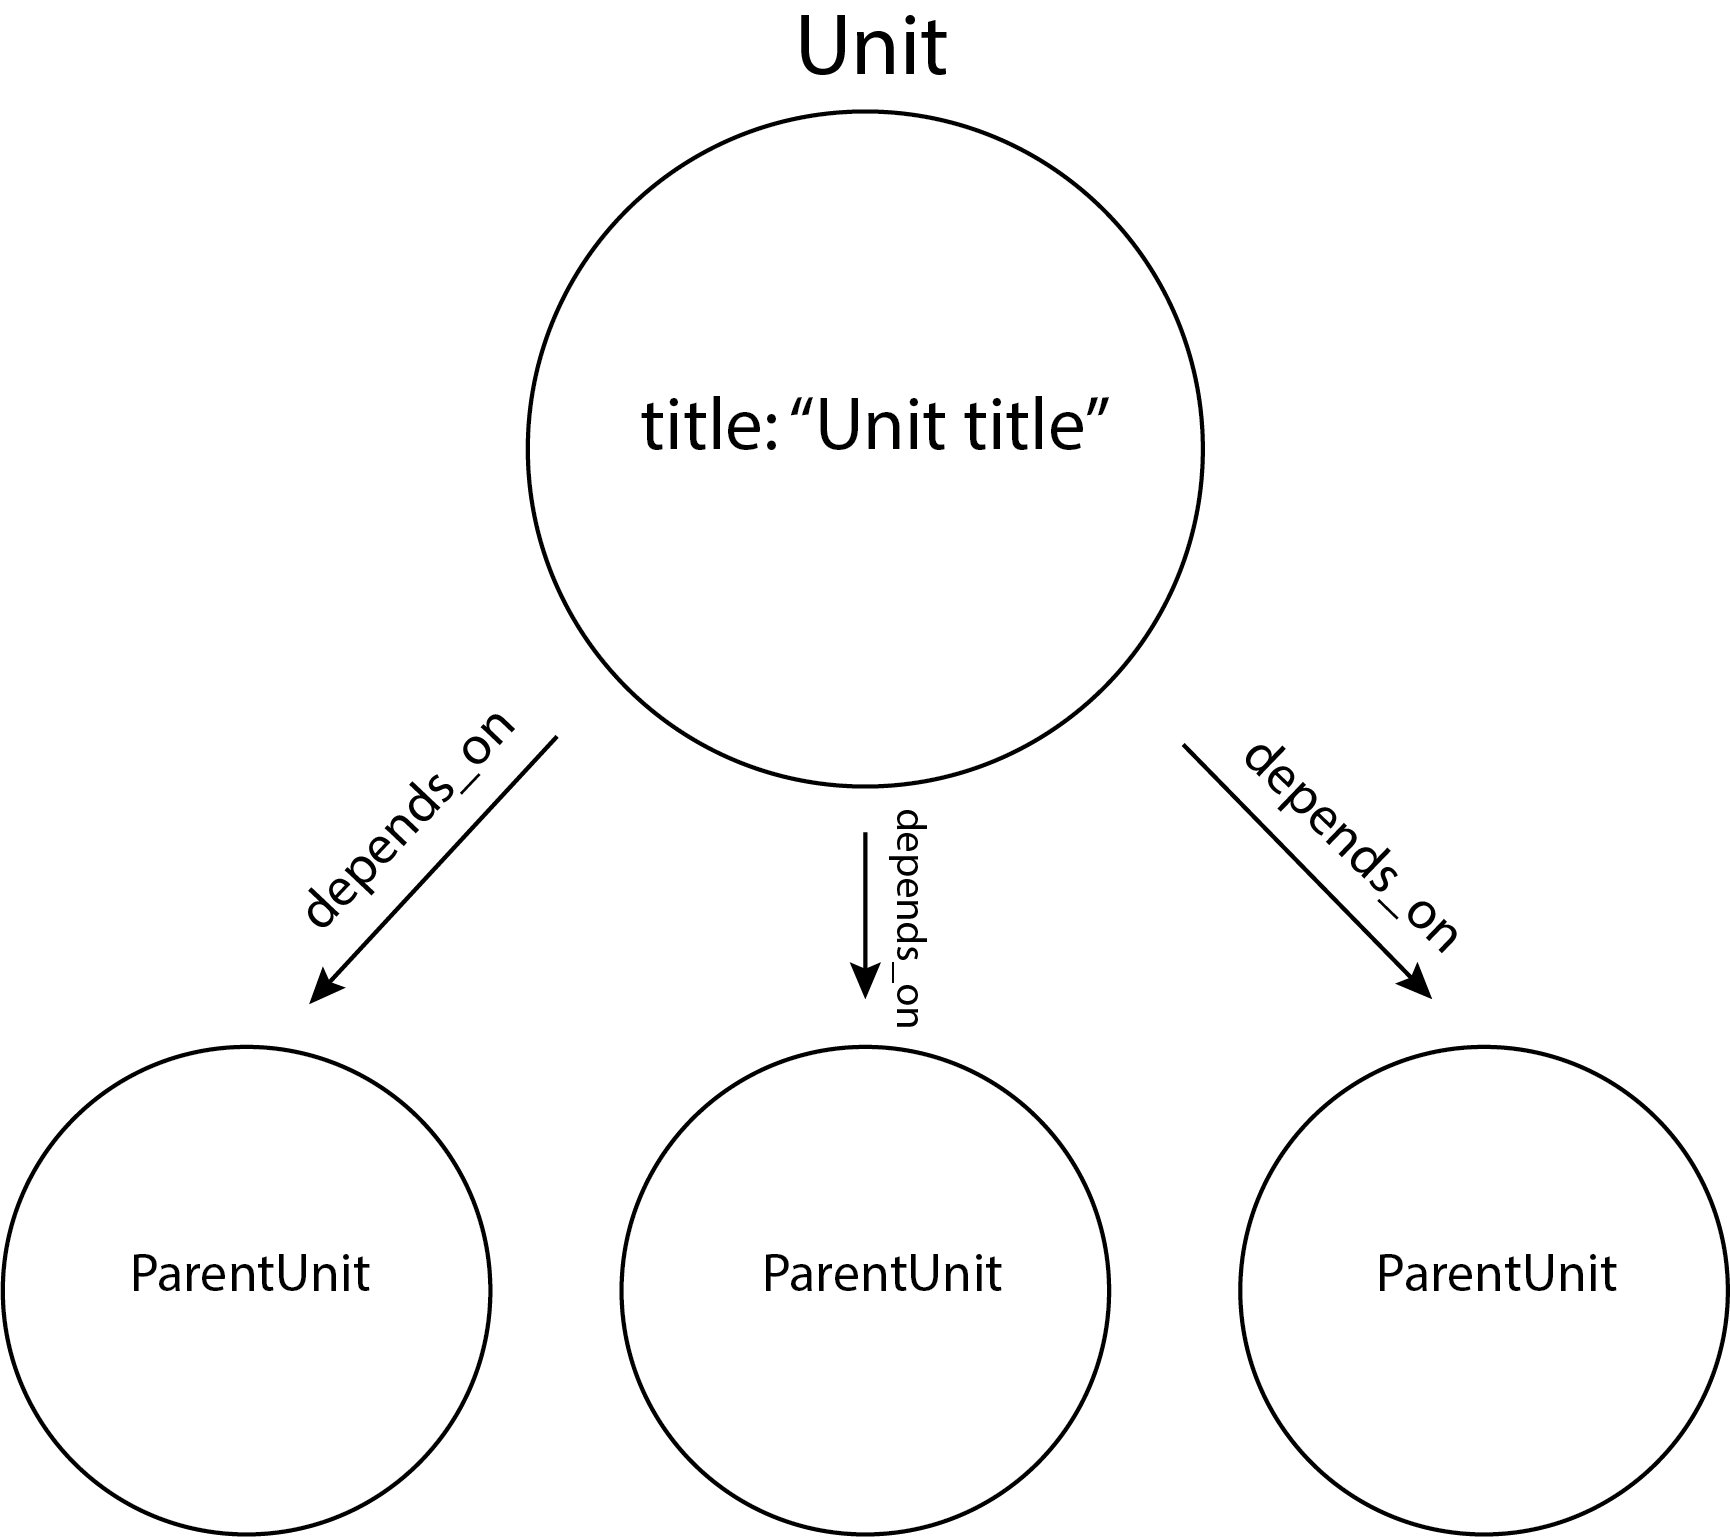
\includegraphics[scale=0.5]{units.png}
    \caption[Unit mapping.]{Unit mapping.}
        
    \label{fig:units}
\end{figure}

The final mapping is for the exercise data type. Exercises have three different possible data types it can depend on. They can depend on a topic, a unit or another exercise. The topic and unit dependency should ideally be the same but for our purposes, both must be satisfied in order for this dependency to be satisfied. In the absence of one, specifically the topic dependency, the other can be used. This is because if the topic dependency is missing for an exercise but unit dependencies are listed, the topic dependency can be generated by traversing the unit dependency mapping for the given units the exercise depends on. The final dependency on exercises is independent of topic or unit. The situation for exercise dependency arises when the results of one exercise are used in another exercise. In this situation, a given exercise should follow immediately after the dependent exercise or after another exercise that shares the same dependency on the same exercise.

Outside of dependency mapping, there is the actual order of the textbook and order of exercises. They can be contained with a DAG much like all the other topics. These are what actually describes how the textbook will actually be structured. These mappings are the only ones that are mutated for the sole purpose of reordering a textbook. There is a base mapping that is initially defined by the author for the first publication of the book. These base mappings should be structured in a way such that all dependencies are satisfied.

Finally it must be formally defined what \textit{satisfying all dependencies} mean. It short, a unit or exercise satisfy all dependencies when all of its dependencies' dependencies are satisfied. For an entity to depend on another entity, it simply means that the parent entity must occur or appear in an earlier point in the dependency mapping tree. Since this is a recursive definition, it must terminate with some sort of base case. This base case is a base unit or topic which is a unit or topic that has no other dependencies. If all other topics, units and exercises that a particular entity has depends on has appeared earlier on in the dependency mapping tree, then it can be said that this entity has all dependencies satisfied.

\subsection{Flow}

For a textbook that is going to be integrated into this dynamic modification flow, several dependency trees/DAGs need to be laid out describing the textbook. Specifically the different orderings as defined by the original author and a consumer and how they interact with one another must be laid out. They are as follows.

\begin{enumerate}
    \item Tree of unit ordering
    \item Tree of exercise ordering 
    \item Tree of unit interdependency $+$ topic dependency \ref{fig:units}
    \item Tree of exercise interdependency $+$ topic or unit dependency
    \item Tree of topic interdependency
\end{enumerate}

Trees 1 and 2 are initially created by the original author in order to define the original ordering of the given textbook. These trees (1 and 2) are the only ones that will ever be modified by the consumer in order to reorder a given textbook. Trees 3, 4 and 5 are defined by the author at the completion of writing the textbook and should not be modified for the current version of the textbook. A modification of trees 3, 4 or 5 should be done to correct a dependency mistake, to add a new entity or to remove an entity. These modifications should result in a new edition of the textbook. Trees 3, 4 and 5 are used in order to validate and confirm that all dependencies are met in trees 1 and 2 for both the original 1 and 2 trees created by the author as well as for when they are modified by the consumer.

The actual workflow is as follows.

\begin{enumerate}
    \item Original author creates trees 1, 2, 3, 4 and 5. Trees 1 and 2 may be generated if trees 3, 4 and 5 are completed.
    \item Adopting institution or instructor specifies the desired ordering of the textbook by modifying tree 1.
        \begin{enumerate}
            \item During this process warnings may be provided to the user if any of their modifications to tree 1 cause a dependency to not be met as defined in trees 3, 4 and 5
        \end{enumerate}
    \item Using trees 3, 4 and 5 as well as the user modified tree 1, tree 2 is generated defining the order of the exercises
        \begin{enumerate}
            \item The adopting institution or instructor can preview the exercise and modify the order in which they may appear.
            \item During this process warnings may be provided to the user if any of their modifications to this newly generate $+$ modified tree 2 cause a dependency to not be met as defined in trees 1, 3, 4 and 5
        \end{enumerate}
    \item The newly generated order in the form of trees 1 and 2 can then be utilized to modify the text and links in the given textbook
\end{enumerate}
